% #############################################################################
% This is Chapter 2
% !TEX root = ../main.tex
% #############################################################################
% Change the Name of the Chapter i the following line
\fancychapter{Fundamental Concepts}
\cleardoublepage
% The following line allows to ref this chapter
\label{chap:back}

This chapter introduces the fundamental technical concepts and architectures underlying open-vocabulary referring segmentation systems.

% #############################################################################
\section{Neural Networks and Deep Learning}

Basic concepts of deep neural networks, convolutional architectures, and optimization techniques.

\begin{figure}[htbp]
\centering
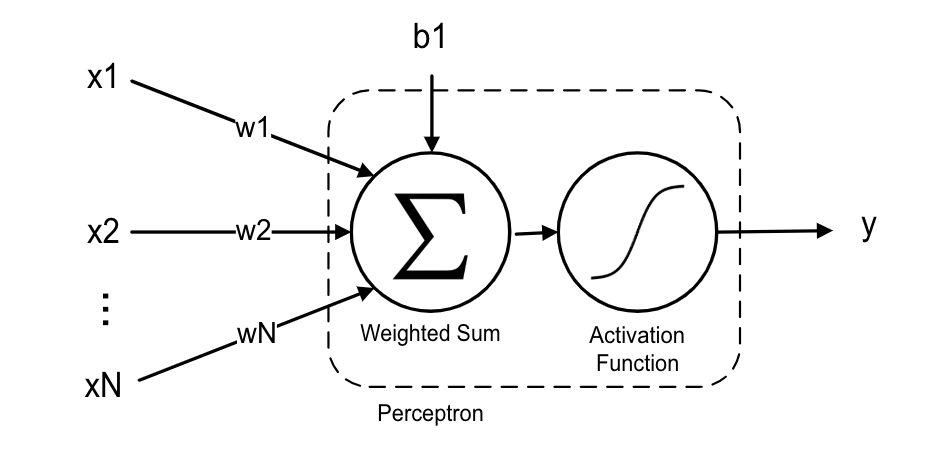
\includegraphics[width=0.8\textwidth]{Images/perceptron.png}
\caption{Perceptron architecture and basic neural network building block.}
\label{fig:perceptron}
\end{figure}

\begin{figure}[htbp]
\centering
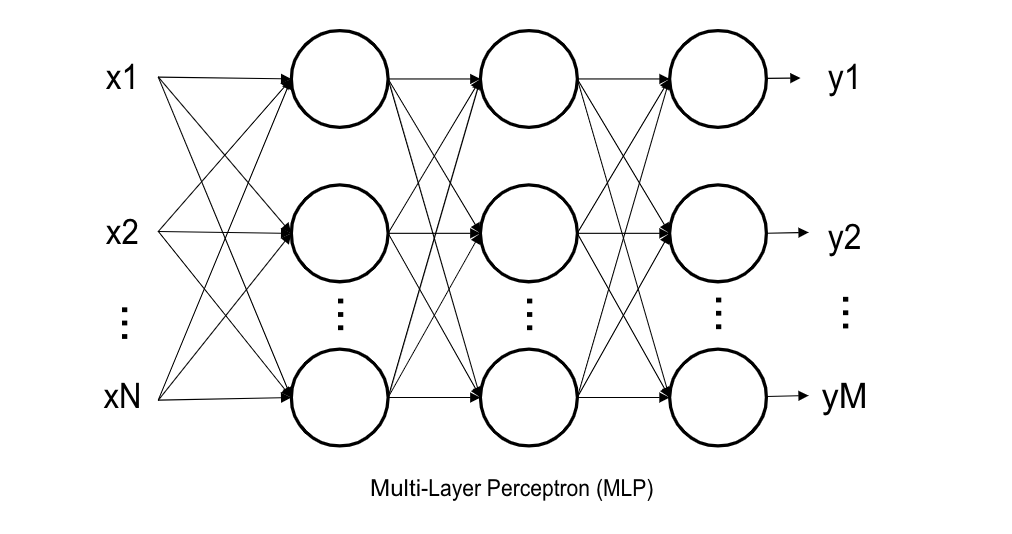
\includegraphics[width=0.8\textwidth]{Images/mlp.png}
\caption{Multi-layer perceptron architecture showing feedforward neural network structure.}
\label{fig:mlp}
\end{figure}

% #############################################################################
\section{Attention and Transformers}

Self-attention mechanisms, encoder-decoder architectures, and positional encoding.

\begin{figure}[htbp]
\centering
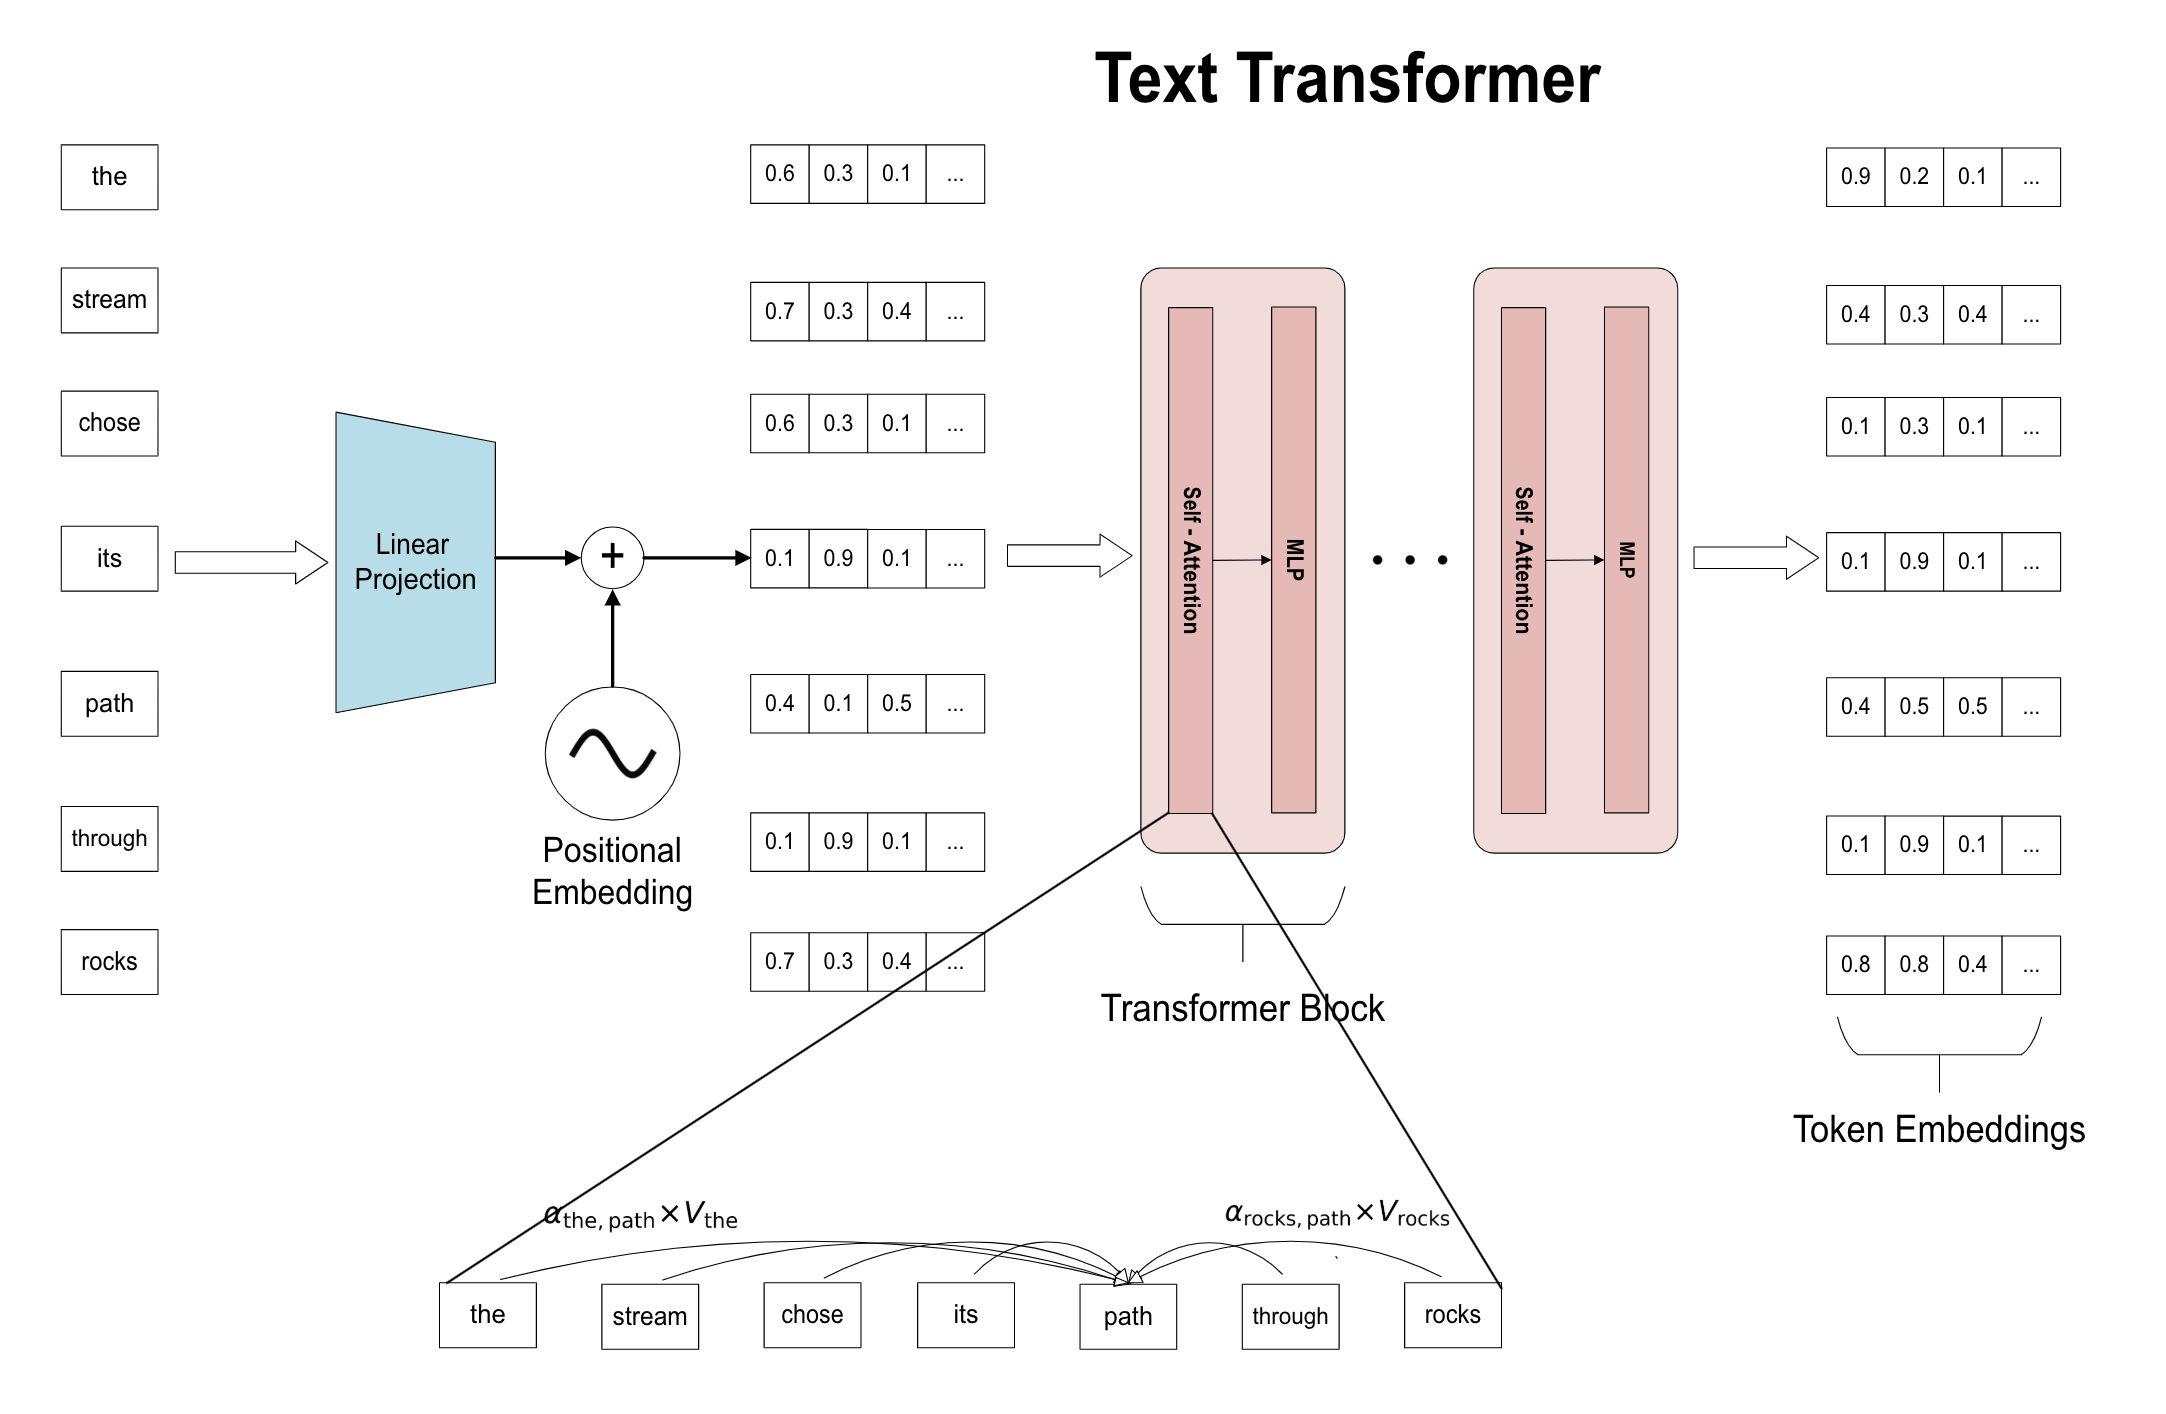
\includegraphics[width=0.8\textwidth]{Images/transformer.png}
\caption{Transformer architecture with self-attention mechanisms and encoder-decoder structure.}
\label{fig:transformer}
\end{figure}

% #############################################################################
\section{Transformers for Computer Vision}

Application of transformer architectures to computer vision tasks and visual understanding.

\begin{figure}[htbp]
\centering
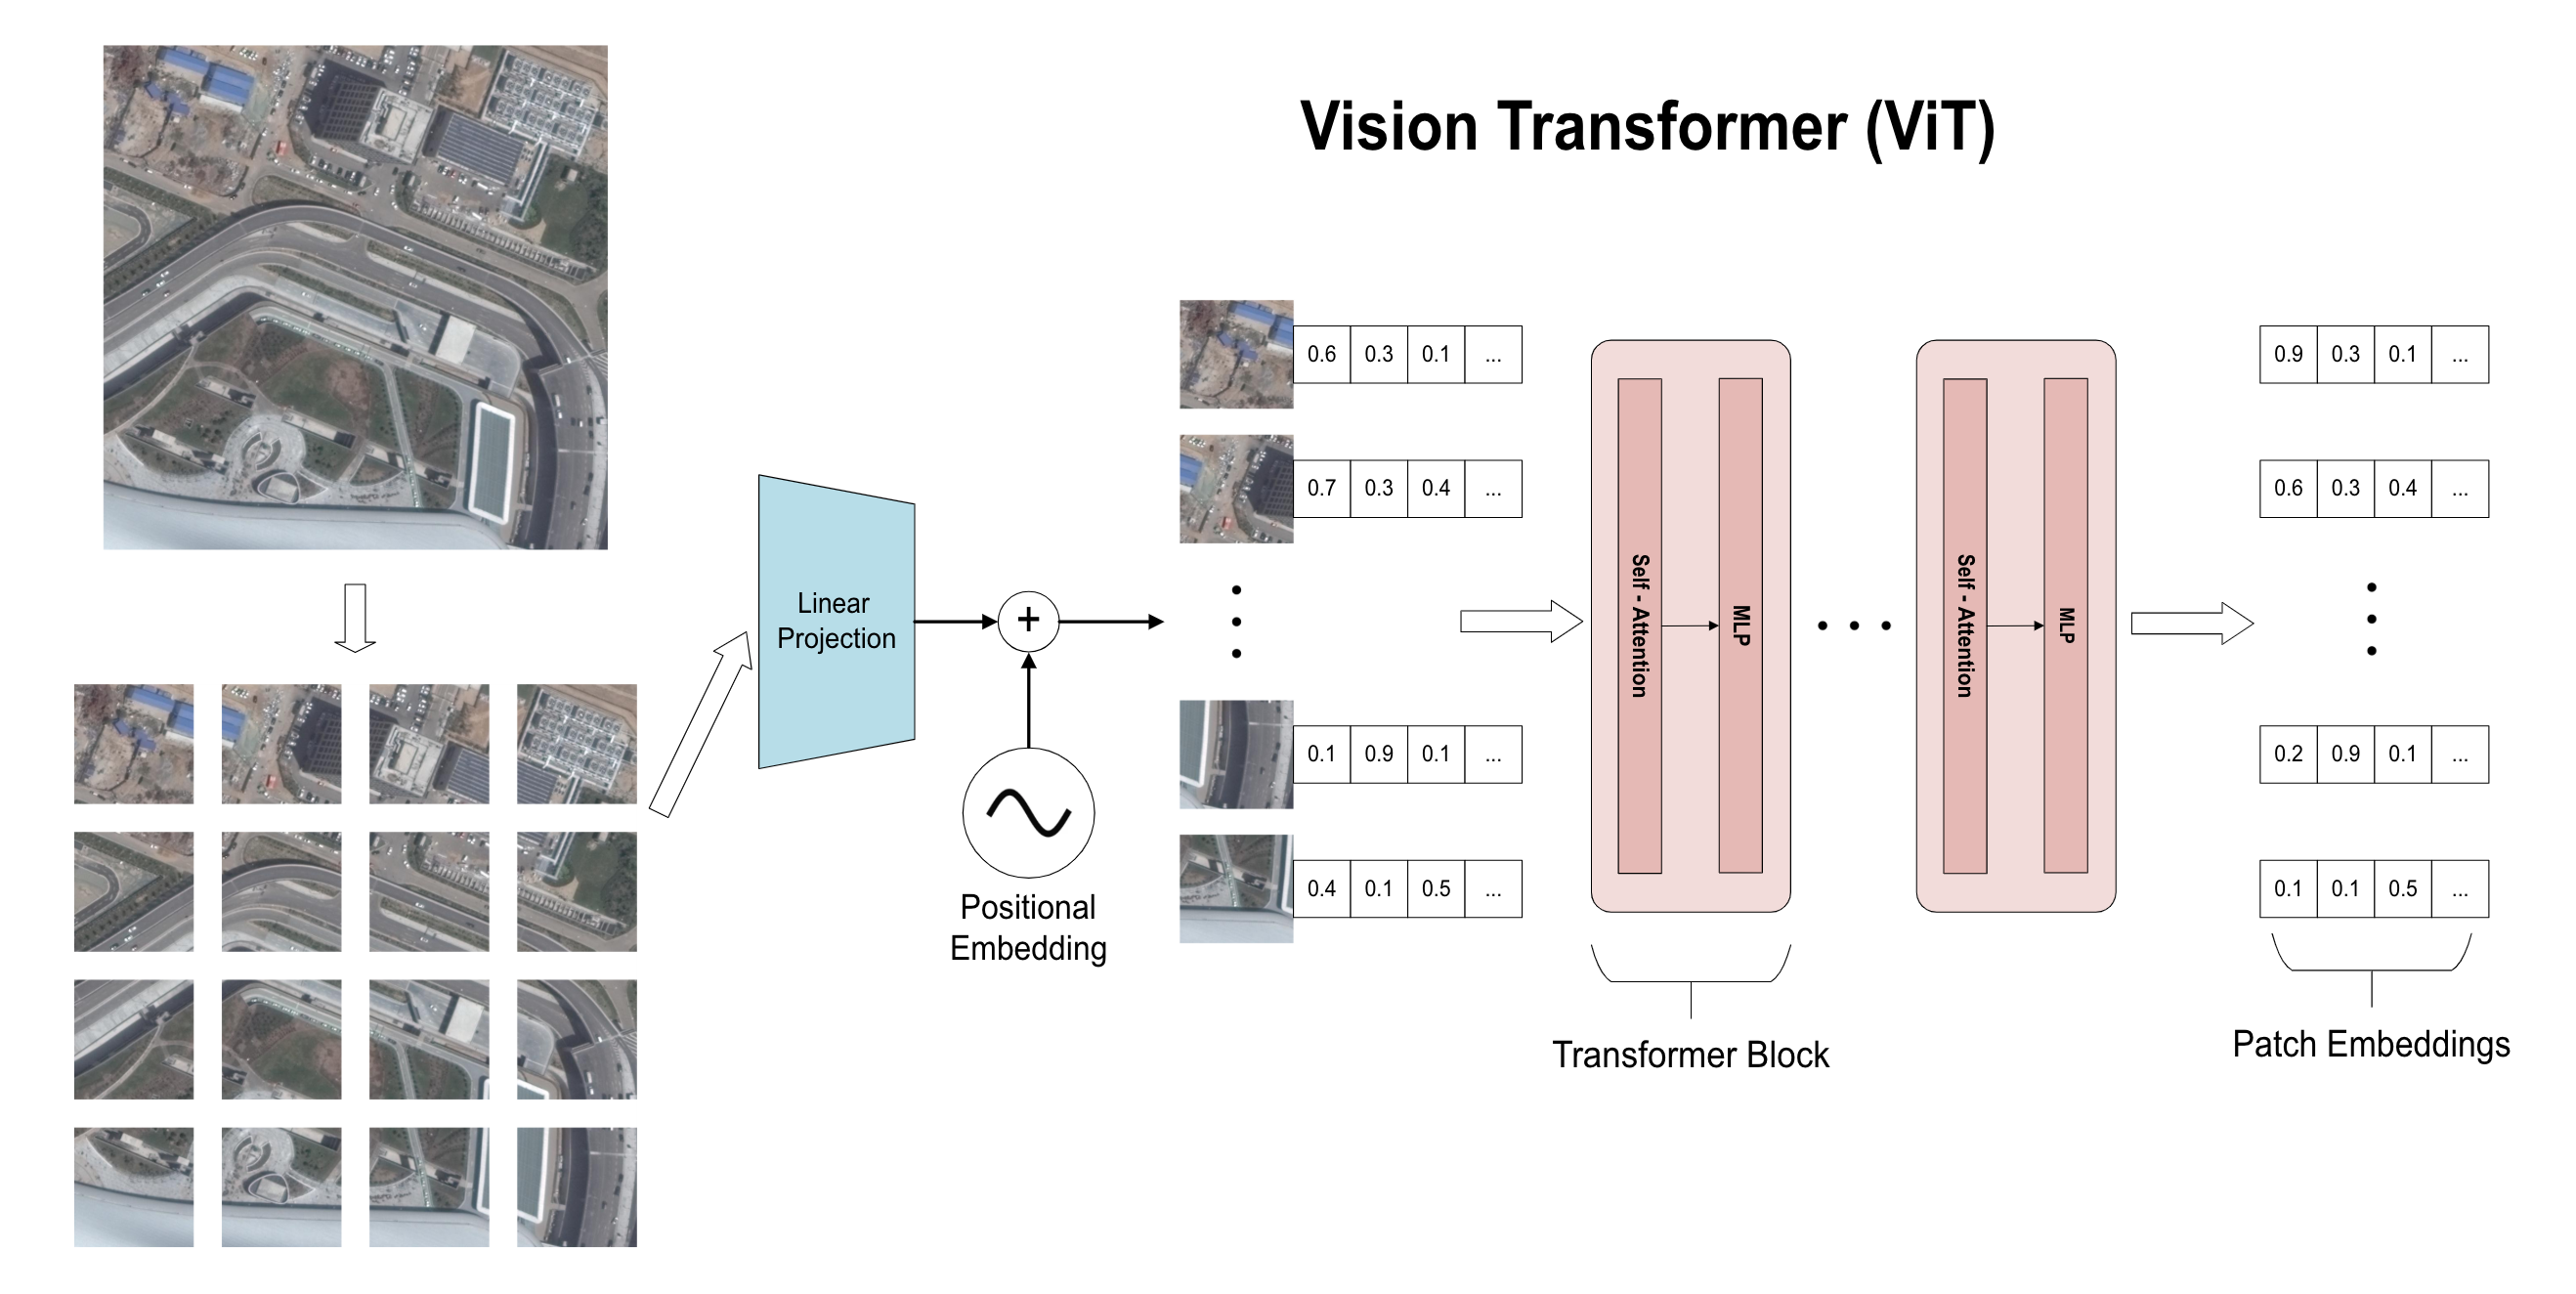
\includegraphics[width=0.8\textwidth]{Images/vit.png}
\caption{Vision Transformer (ViT) architecture for image classification and feature extraction.}
\label{fig:vit}
\end{figure}

% #############################################################################
\section{Image Segmentation}

Deep learning approaches for image segmentation tasks and methodologies.

% #############################################################################
\section{Vision-Language Models}

Multimodal architectures that process both visual and textual information.

\subsection{CLIP and Visual-Language Learning}

Contrastive Language-Image Pre-training model architecture and visual-language learning methodologies.

\subsection{Large Language Models}

Foundation models for natural language understanding and generation in multimodal contexts.

\begin{figure}[htbp]
\centering
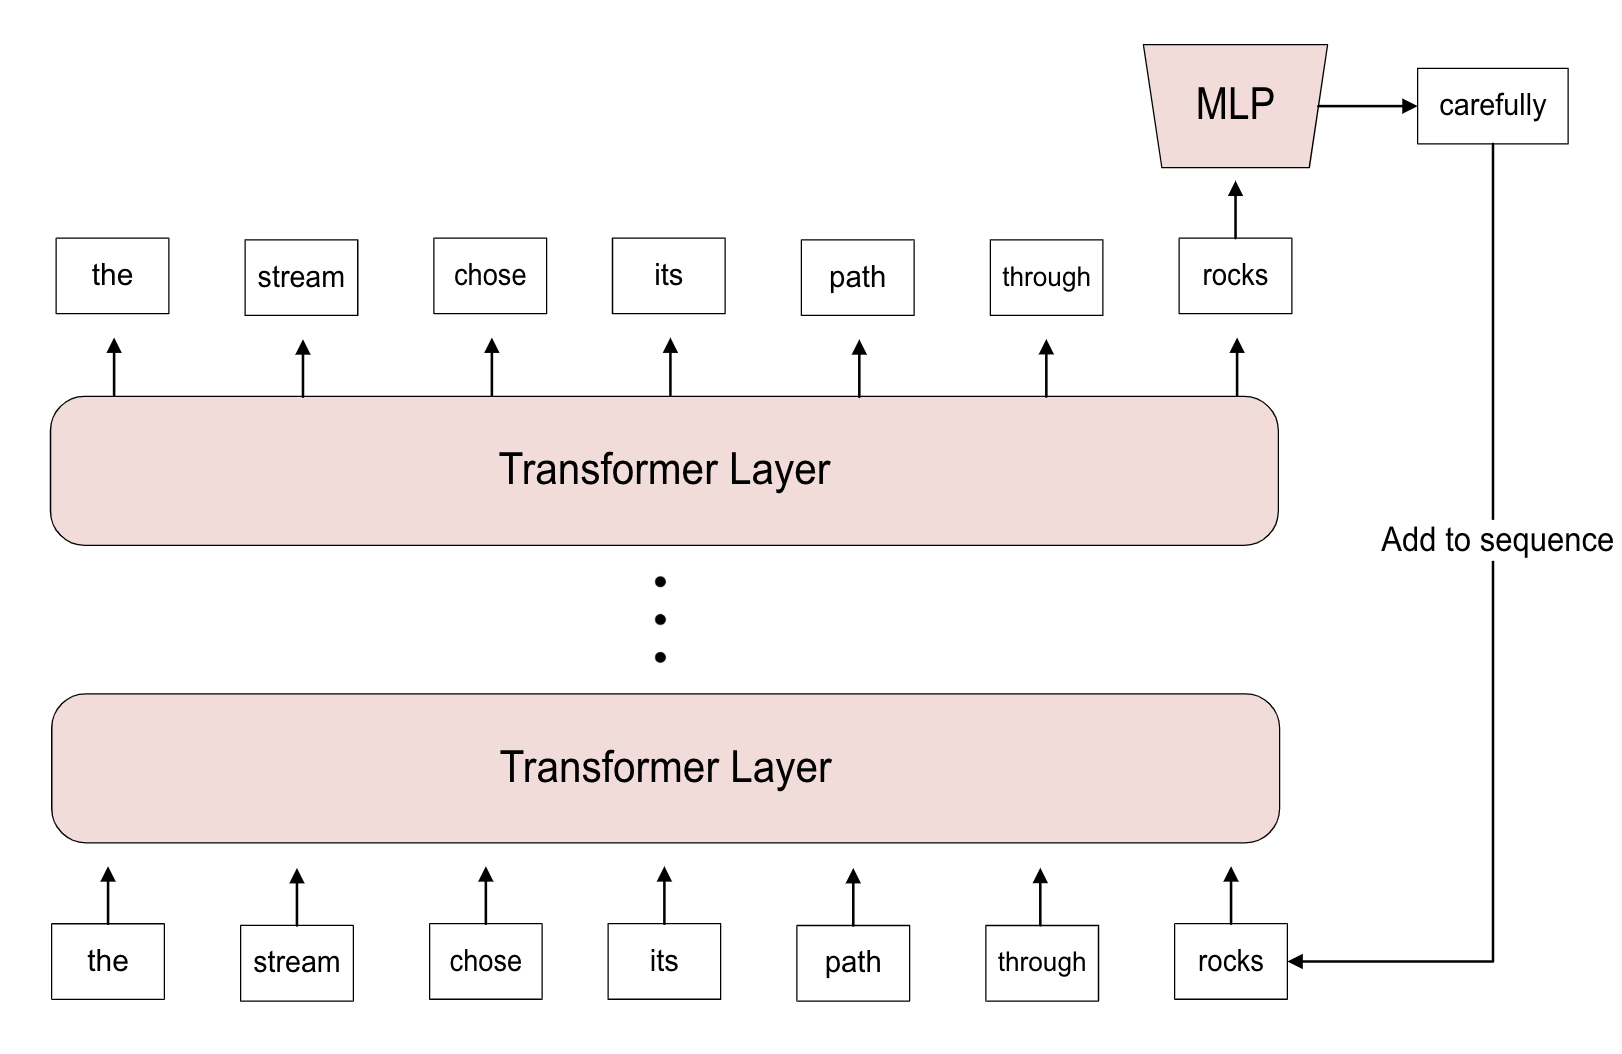
\includegraphics[width=0.8\textwidth]{Images/gpt.png}
\caption{GPT autoregressive language model architecture showing the transformer decoder stack with next-token prediction and feedback mechanism.}
\label{fig:gpt}
\end{figure}